\documentclass[10,a4paper]{article}
\usepackage[utf8]{inputenc}
\usepackage{amsmath}
\usepackage{amsfonts}
\usepackage{amssymb}
\usepackage{graphicx}
\title{ASR2: TP12}
\author{Vincent RÉBISCOUL}
\begin{document}
\maketitle
\section*{Exercice 1}
\subsection*{Question 1}
\begin{center}
  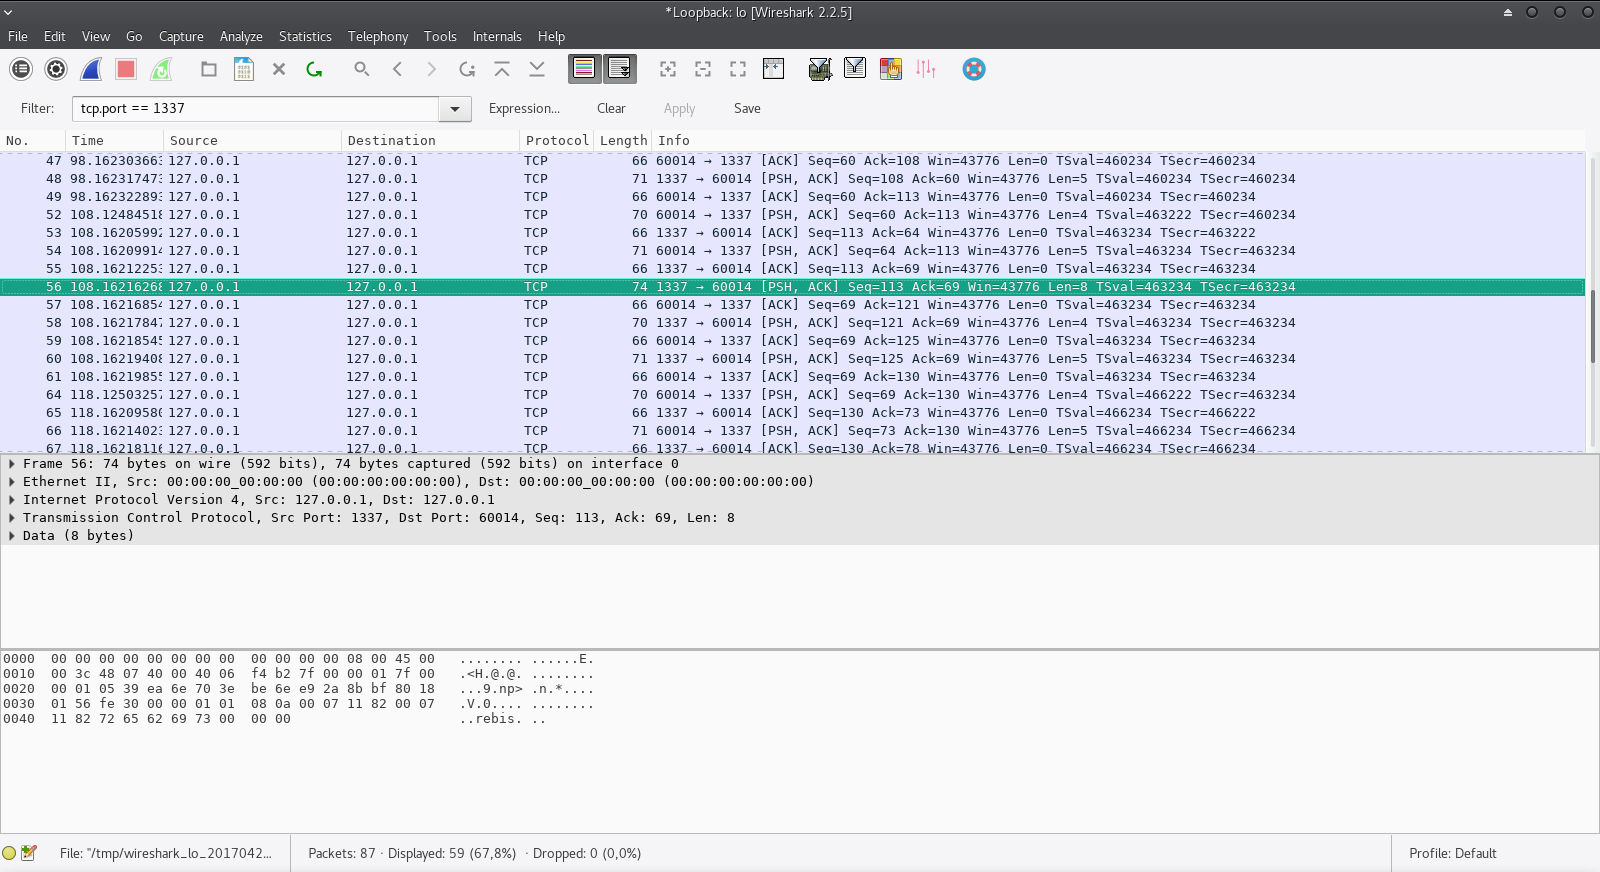
\includegraphics[width=15cm]{exo1_1.png}
\end{center}
\subsection*{Question 2}
C'est l'établissement de la connection entre le serveur et le client.

\subsection*{Question 3}
\subsubsection*{CLIENTHELLO}
On peut voir le ``Hi everyone I'm here'' sur la capture.
\begin{center}
  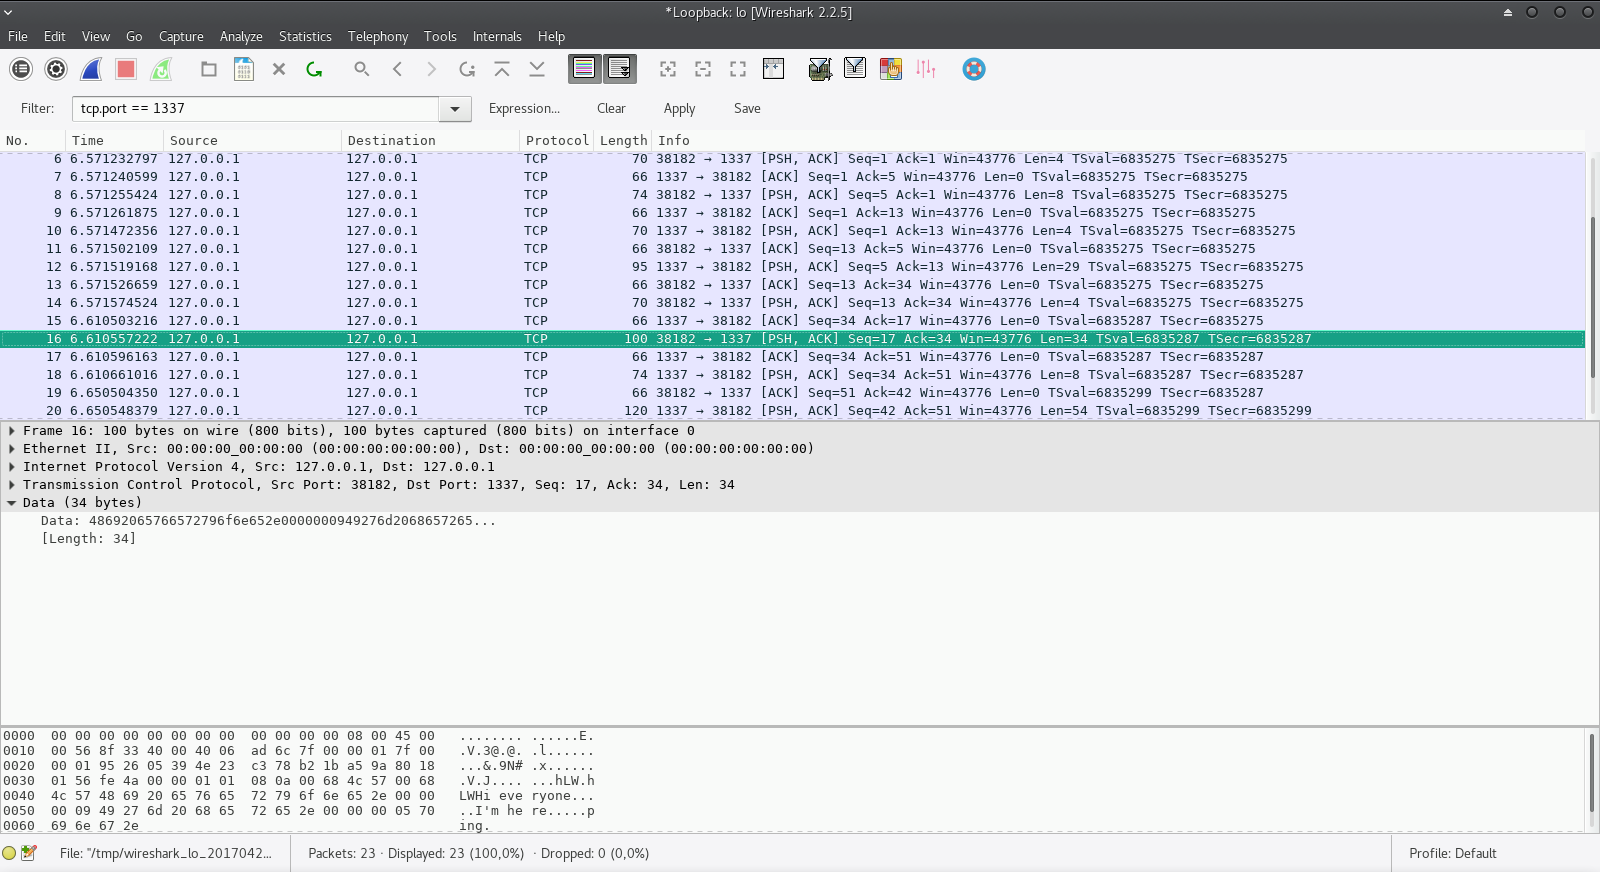
\includegraphics[width=15cm]{exo1_3_clienthello.png}
\end{center}

\subsubsection*{SERVERHELLO}
On peut voir le ``Welcome to this server''  sur la capture.
\begin{center}
  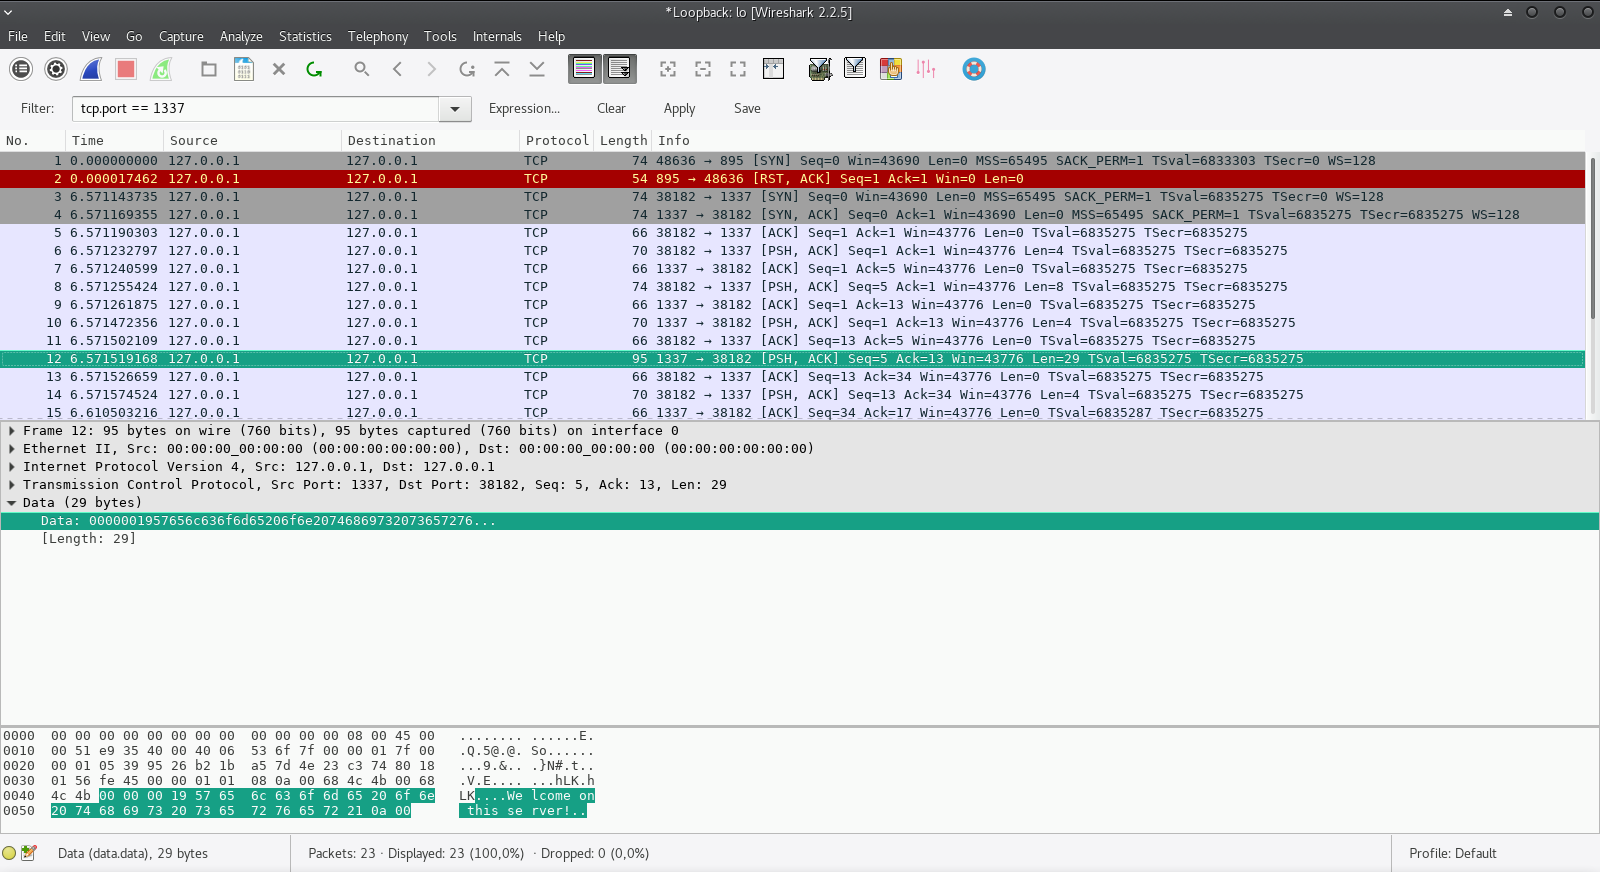
\includegraphics[width=15cm]{exo1_3_serverhello.png}
\end{center}

\subsection*{Question 4}
\subsubsection*{CLIENTMSG}
On peut voir le ``ping'' sur la capture.
\begin{center}
  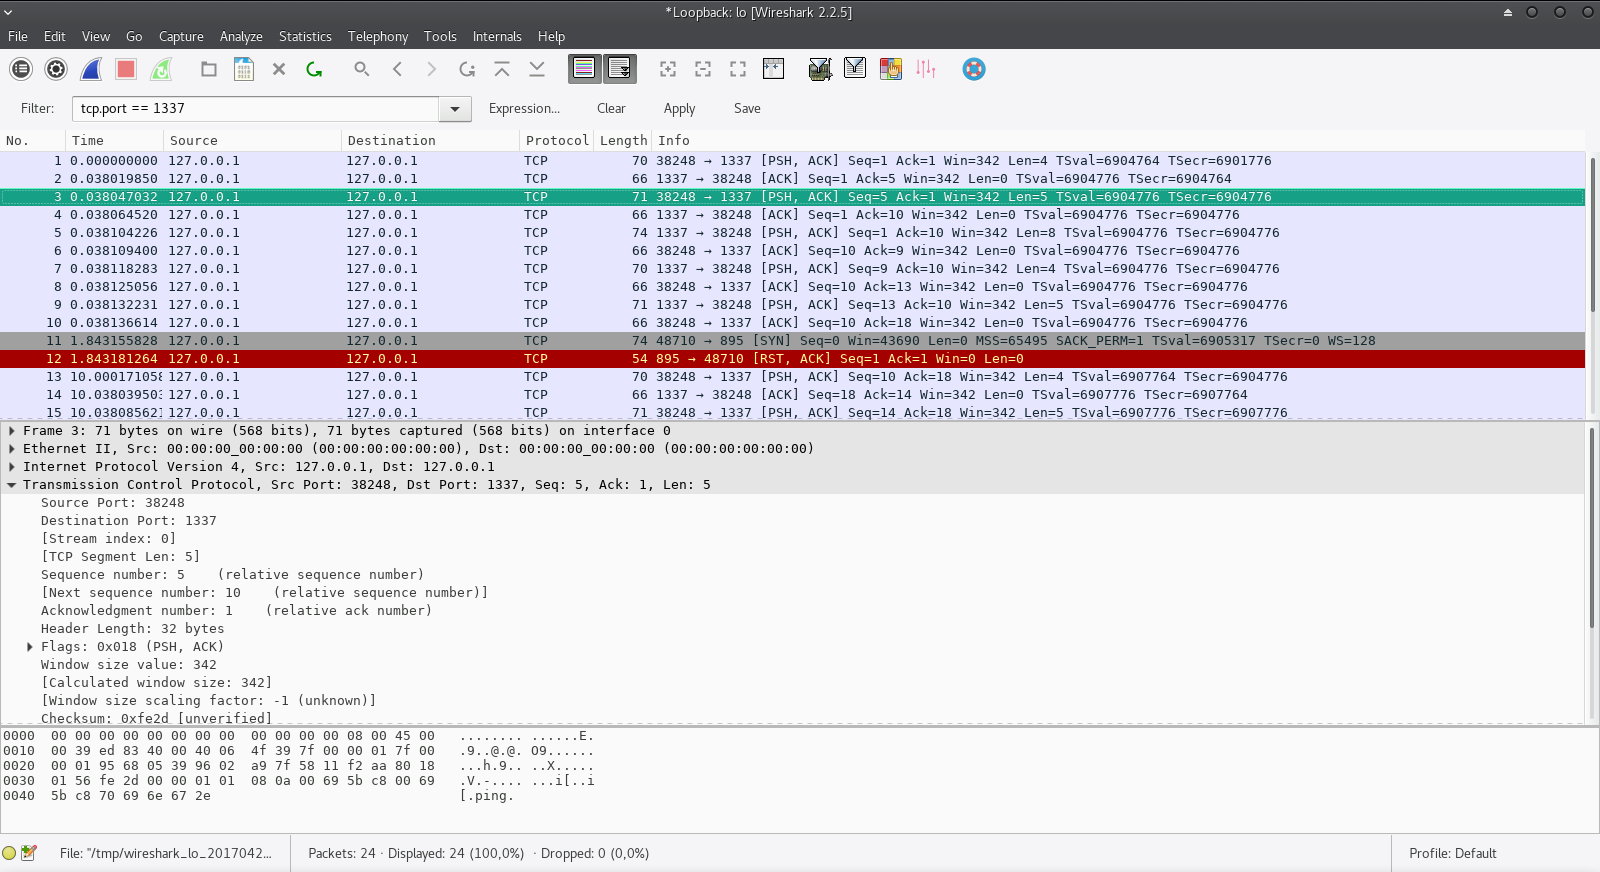
\includegraphics[width=15cm]{exo1_4_clientmsg.png}
\end{center}

\subsubsection*{SERVERMSG}
On peut voir le ``yo'' sur la capture.
\begin{center}
  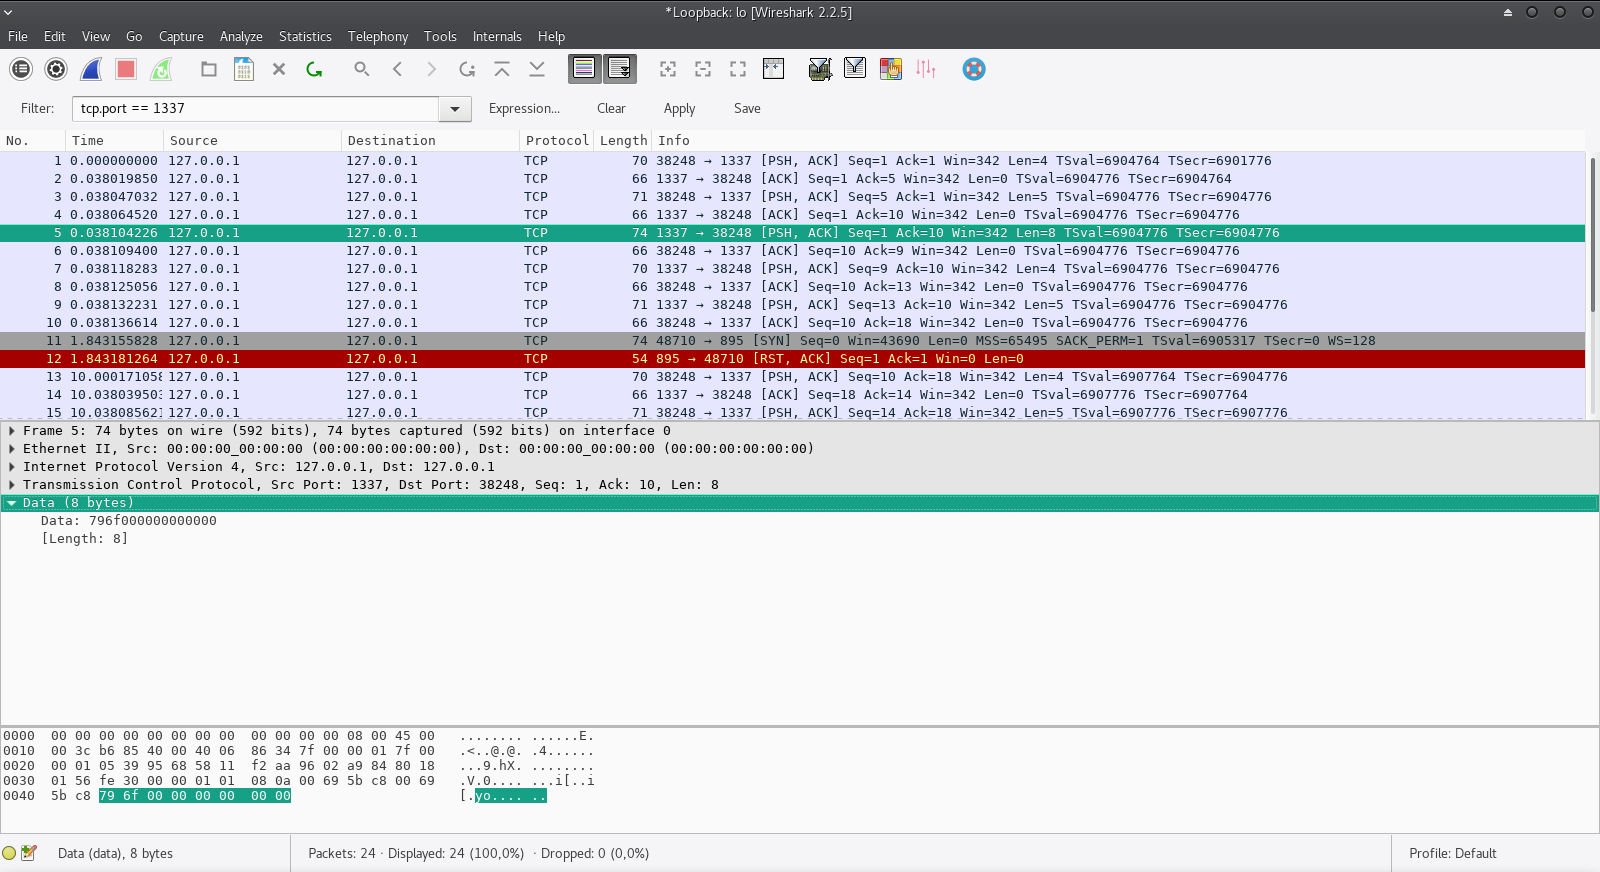
\includegraphics[width=15cm]{exo1_4_servermsg.png}
\end{center}


\section*{Exercice 2}
\subsection*{Question 1}
\begin{center}
  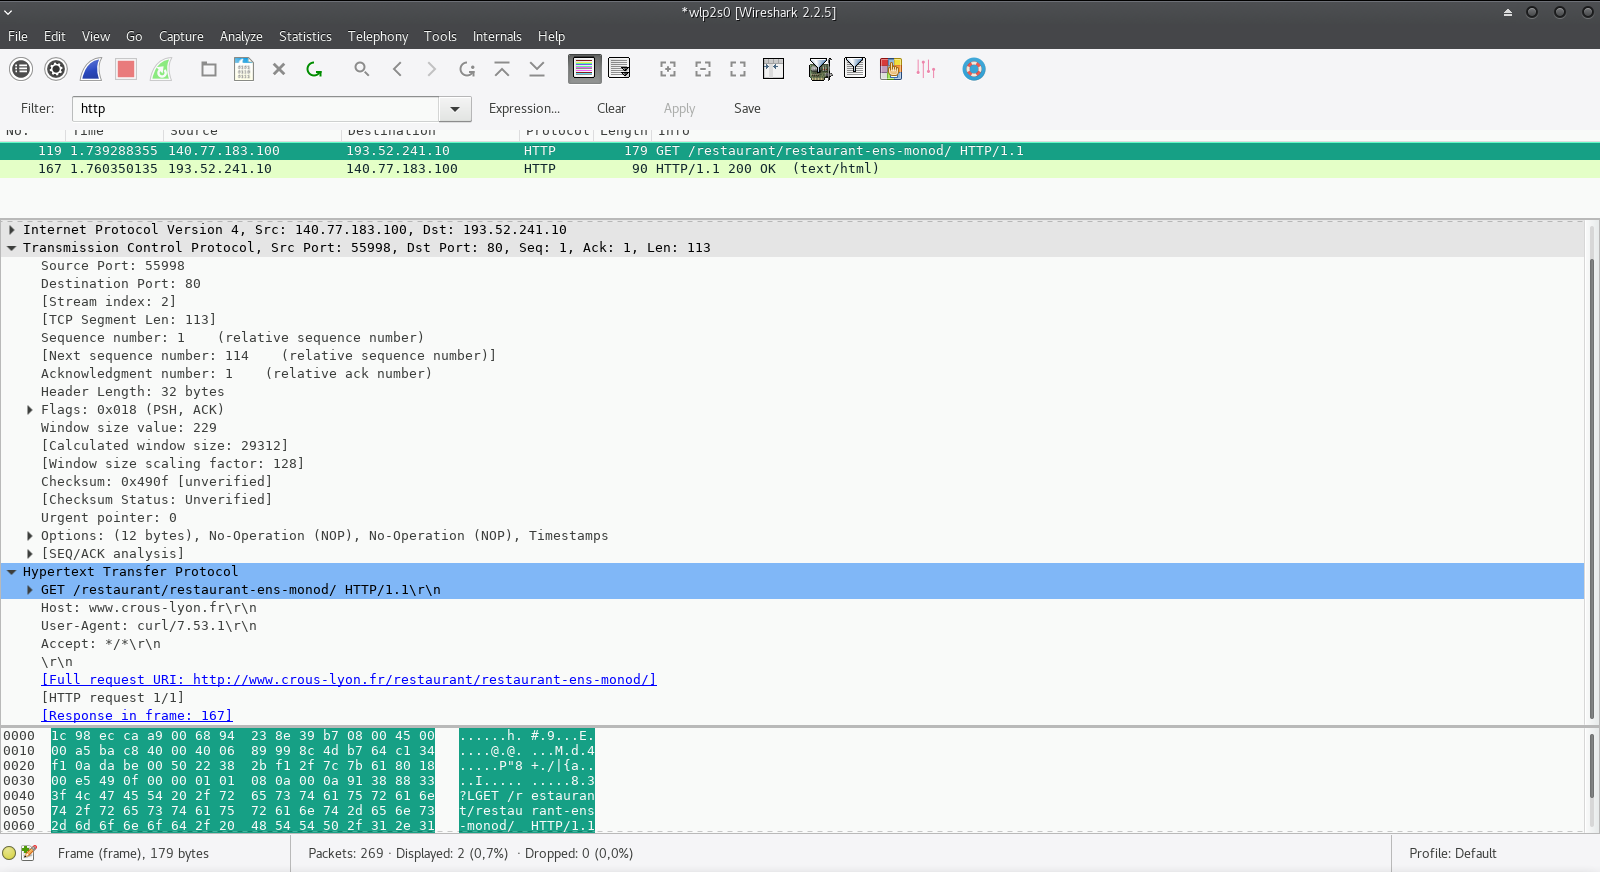
\includegraphics[width=15cm]{exo2_1.png}
\end{center}
On voit une requête ``GET'' qui demande une page web, on a l'host qui est le serveur où l'on va chercher la page et le user-agent qui indique quel programme on a utilisé.

\subsection*{Question 2}
\begin{center}
  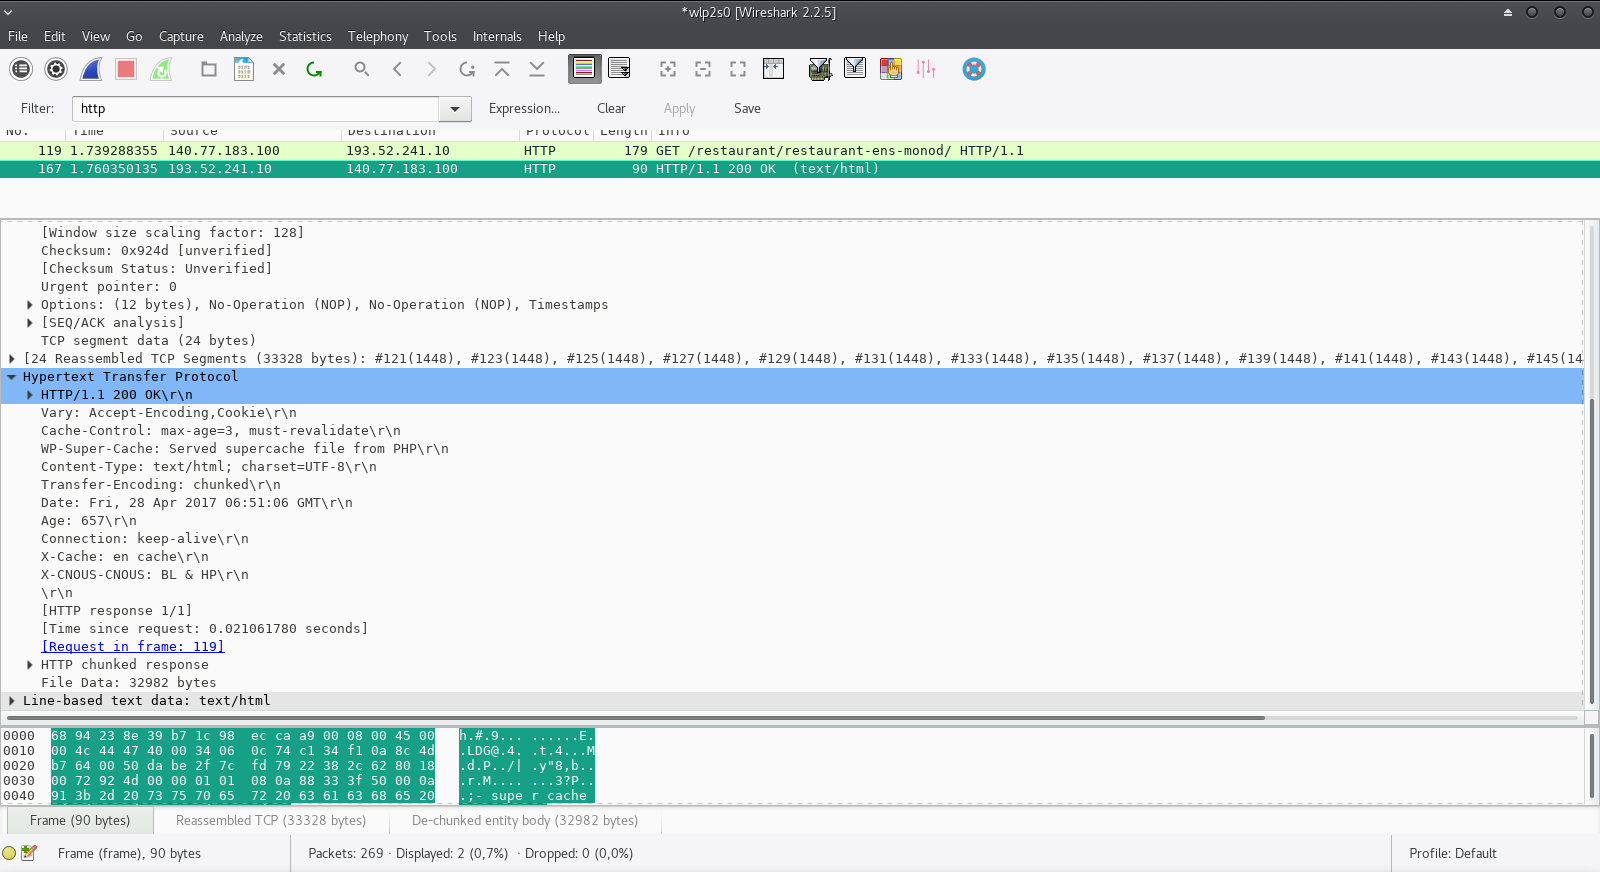
\includegraphics[width=15cm]{exo2_2.png}
\end{center}
On peut voir différents champs tel que ``content-type'' qui indique l'encodage et le type de fichier (ici un fichier html). On peut voir dans ``transfer-encoding'' que le fichier est ``chunked'', c'est à dire découpé en plusieurs ``chunks''. En bas de la capture d'écran, on peut voir ``lined-based text data'', c'est là où se trouve le code HTML.

\subsection*{Question 3}
La commande ne marche pas. curl n'arrive pas à vérifier le certificat SSL, plus précisement curl n'arrive pas à avoir le certificat local.

\subsection*{Question 4}
Non, je n'arrive pas à trouver une requête HTTP, cela est du au fait que l'on soit en HTTPS. On peut néanmoins observer des échanges avec le protocol TLS, ces échanges sont donc cryptés.

\subsection*{Question 5}
Cela permet à curl d'effectuer des requêtes non-sécurisée. On ne vérifie plus les certificats SSL. C'est donc évidemment peu recommandé...

\section*{Exercice 3}
\subsection*{Question 1}
\begin{itemize}
\item \underline{ARP:} C'est le protocol qui fait le lien entre adresse MAC et adresse IP local. On voit beaucoup de requête ``Who has''
\item \underline{DNS:} Protocol qui fait le lien entre URL et adresse IP. On demande à un serveur quel est l'IP du serveur www.archlinux.org (par exemple) et le serveur DNS nous renvoie l'IP.
\item \underline{MDNS:} Même chose mais ne requiert pas de serveur DNS. Cela est utilisé pour les petits réseaux.
\item \underline{DHCP:} Protocol qui permet l'appareillement entre une adresse MAC et une adresse IP. Lorsque l'on connecte une machine sur un réseau, on va demander au réseau une adresse IP local via le protocol DHCP.
\item \underline{BROWSER:} C'est un protocol de Windows visiblement. Il utilise massivement le broadcast.
\item \underline{DP-LSP-DISC:} C'est un protocol de Dropbox apparemment. J'imagine que cela permet d'utiliser le logiciel dropbox. Ce protocol utilise aussi beaucoup les broadcasts.
\end{itemize}

\end{document}